\begin{appendices}
\chapter{Le Web sémantique}
\label{annexe:semantic-web}
% TODO appendix parts

% What is semantic web?

% Le Web tel que nous le connaissons aujourd'hui est encore conforme
% à la vision initial

% Le Web a été conçu principalement pour une utilisation par les
% humains. Néanmoins, il existe un effort visant à automatiser son
% utilisation et pour apporter le Web plus accessible pour les
% machines.

% \cite{bartalos2011effective} The Web was primarily designed for use
% by humans. Nevertheless, there is an ef- fort to automate its use
% and bring the Web more accessible for machines. This has brought
% forward the need for machine processable representations of
% semantically rich information. This has brought forward the need for
% machine processable representations of semantically rich
% information: a vision at the heart of the Semantic Web

Dans un premier temps, on va essayer de clarifier la notion d'un
services Web sémantique, puis étudie les langages émergeants qui
permettent de décrire ce type de services Web.

L'objectif premier du Web sémantique est de définir et lier les
ressources du Web afin de simplifier leur utilisation, leur
découverte, leur intégration et leur réutilisation dans le plus grand
nombre d'applications \cite{berners2001semantic}. Le Web sémantique
doit fournir l'accès à ces ressources par l'intermédiaire de
descriptions sémantiques exploitables et compréhensibles par des
machines. En effet, Les technologies du Web sémantique complètent le
Web actuel avec des outils sémantiques. Il ne s'agit donc pas de créer
un nouveau Web ou un Web séparé de l'existant : ce Web de données
repose entièrement sur les technologies et concepts qui ont fait le
succès du Web tel que nous le connaissons aujourd'hui
\cite{bertails2010web}.

La réalisation du Web sémantique trouve ces racines dans le
développement des langages de balisage inspiré par des travaux issue
de la communié AI \cite{mcilraith2001semantic}, tels que \textsc{OIL}
\cite{fensel2001oil}, \textsc{DAML+OIL} \cite{horrocks2002daml+oil} et
\textsc{DAML+OTN} \cite{mcguinness2003daml} (ces deux derniers
langages sont parties de la famille \acrshort{daml}).

  % TODO refactor
Ces langaes ont une sémantique bien définies et permettent le balisage
et la manipulation des taxonomique complexe et Des relations logiques
entre les entités sur le Web. \cite{fensel2000creating}

% %!TEX root = ../main.tex
\begin{figure}[h]
    \centering
    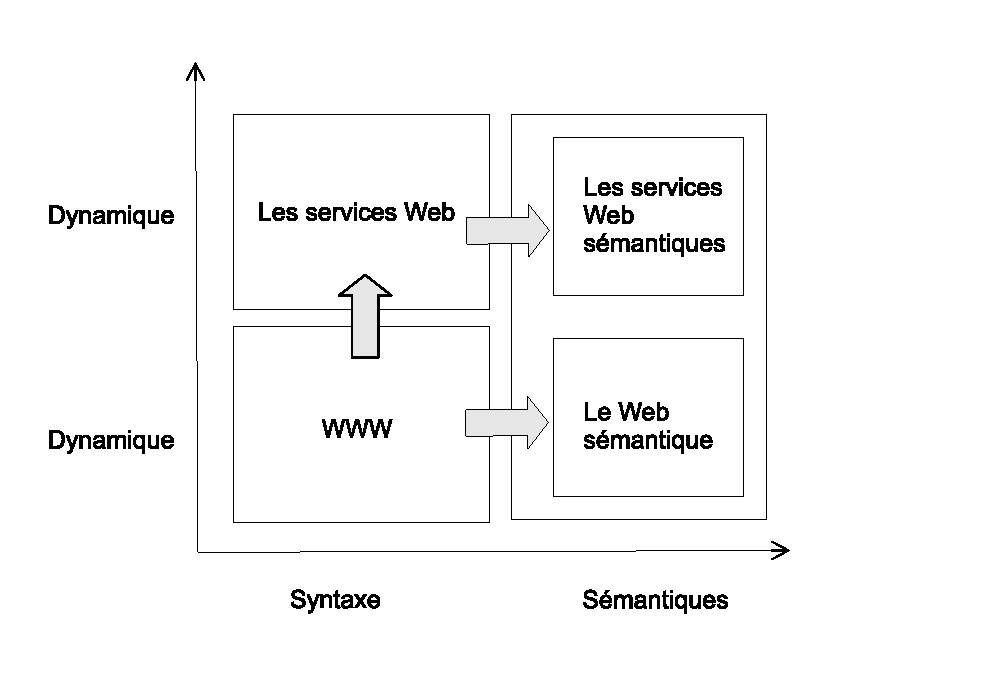
\includegraphics[width=1\textwidth]{figs/3w_to_sws.eps}
    %TODO translate
    \caption{Web evolution to Semantic Web services \cite{fensel2002semantic}.}
    \label{fig:3w_to_sws}
\end{figure}

Cette description repose sur des ontologies. Selon Gruber
\cite{gruber1993translation}, une ontologie est une spécification
explicite d'une conceptualisation. Une conceptualisation est un modèle
abstrait qui représente la manière dont les personnes conçoivent les
choses réelles dans le monde et une spécification explicite signifie
que les concepts et les relations d'un modèle abstrait reçoivent des
noms et des définitions explicites. Le Web sémantique est devenu un
domaine à part entière, preuve en est la création en 2001 du groupe de
travail sur ce sujet par le \textsc{W3C}.

\chapter{Les mesures de similarité}
\label{annexe:similarity-measurement}

L'objectif des mesures de similarité sémantique est d'évaluer la
proximité sémantique entre les concepts (auxquels les termes des
requêtes et documents sont rattachés). Et comme le matching des
services web revient à trouver les similarités entre les concepts
décrivant les propriétés des services web, nous avons jugé utile
d'explorer les différentes méthodes de recherche de similarité
utilisées dans le domaine de la recherche d’information, en
particulier.

\begin{mydef}[Similarité entre concepts]
  Une similarité $\sigma$: C $\times$ C $\rightarrow$ [0,1] est une
  fonction de couples de concepts vers un nombre compris entre 0 et 1
  exprimant le degré de similarité entre deux concepts, tel que:
  \SpecialItem
  \begin{itemize}
  \item x $\in$ C, $\sigma$(x,x) = 1
  \item x, y $\in$ C, $\sigma$(x,y) = $\sigma$(y,x)
  \end{itemize}
\end{mydef}

Les ontologies définissent les propriétés des concepts et les
relations entre concepts. Une de ces relations est utilisée dans notre
application est \textsc{is–a} (est-un). Cette relation est utilisée
pour extraire des taxonomies à partir des ontologies

\begin{mydef}[Similarité basée sur la taxonomie]
  Soit C l'ensemble de concepts définis dans une ontologie. On dit que
  T est une taxonomie et on écrit T(C, $\leq$) tel que c $\leq$ c'
  signifie que c \textit{is–a} c' (le concept c est subsumé par le
  concept).
\end{mydef}

De nombreuses approches ont été proposées pour évaluer la similarité
sémantique entre deux concepts. Ces approches se divisent en trois
catégories [Sli, 2006]: les approches basées sur les arcs, les
approches basées sur le contenu informationnel et les approches
hybrides.

\section{Mesures de similarité sémantique}
\label{sec:semantic-sim}

De nombreuses approches ont été proposées pour évaluer la similarité
sémantique entre deux concepts. Ces approches se divisent en trois
catégories [Sli, 2006]: les approches basées sur les arcs, les
approches basées sur le contenu informationnel et les approches
hybrides.

  \subsection{Approches basées sur les arcs}
  \label{sec:semantic-sim:arcs}

  Le calcul des distances dans l’ontologie est basé sur un graphe de
  spécialisation des objets.  Dans chaque graphe, la distance de
  l’ontologie doit être caractérisée par le plus court chemin qui fait
  intervenir un ancêtre commun ou le plus petit généralisant,
  connectant potentiellement deux objets à travers des descendants
  communs. Parmi les travaux classifiés sous cette bannière on trouve:\\

  \renewcommand{\descriptionlabel}[1]{\hspace{1cm}\textbullet~\textsf{#1}}
  \begin{itemize}
  \item [la Mesure de Wu \& Palmer] Basée sur le principe suivant :
    Etant donnée une ontologie $\Pi$ formée par un ensemble de nœuds
    (Figure 28). R est la racine, X et Y les deux éléments de
    l’ontologie dont nous allons calculer la similarité. Le principe
    de calcul de similarité est basé sur les distances (N1 et N2) qui
    séparent les nœuds X et Y du nœud racine et la distance qui sépare
    le concept subsumant (CS) de X et de Y du nœud R.

    La mesure de Wu et Palmer est définie par la CS formule suivante:
  
    \begin{equation}
      \label{wu_palmer}
      Sim(x,y) = 2 *  \frac{N}{N_{1} + N_{2} + N_{3}}
    \end{equation}\\

    La mesure de [WuP, 1994] est intéressante mais présente une
    limite, cependant, avec cette mesure on peut obtenir une
    similarité plus élevée entre un concept et son voisinage par
    rapport à ce même concept et un concept fils, ce qui est inadéquat
    dans le cadre de la recherche de l’information.\\

  \item [La mesure de Zargayouna]
    Cette mesure de similarité est inspirée de celle de Wu-Palmer
    favorisant les concepts se trouvant dans la même hiérarchie par
    rapport au voisinage. Le lien père-fils est ainsi privilégié xpar
    rapport aux autres liens de voisinage en adaptant la mesure de
    Wu-Palmer. L'adaptation de la mesure est faite au travers de la
    fonction de calcul du degré de spécialisation d'un concept appelé
    spectre (spec) qui mesure sa distance par rapport à l'anti-racine.

    \begin{equation}
      \label{zargayouna}
      Sim(x,y)= 2 * \frac{N}{N_{1} + N_{2} + 2 * N + 2 * Spec(x,y)}
    \end{equation}\\
      
    Où $Spec(x,y)=N_{1}*N_{2} *N_{3}$, tel que $N_{3}$ correspond au
    nombre maximum d'arcs qui séparent le plus petit ancêtre commun du
    concept \textit{virtuel} représentant l'anti-racine, $N_{1}$ et
    $N_{2}$ séparent les nœuds $x$ et $y$ du nœud racine.\\
  \end{itemize}



  

  



  



  La mesure de Resnik


  \subsection{Approches basées sur le contenu informationnel}
  \label{sec:semantic-sim:ci}

  La mesure de Resnik

  La mesure de Lin

  \subsection{Approches hybrides}
  \label{sec:semantic-sim:hybrides}  

  Mesure de Jiang et Conrath 


\section{Mesures de similarité syntaxique}
\label{sec:syntactic-sim}

  \subsection{Approches basées sur les chaînes de caractères}
  \label{sec:syntactic-sim:string}

  La similarité de Jaccard

  Distance de Jaro

  Distance Jaro Winkler

  Distance de Bigram

  \subsection{Les approches basées sur les tokens}
  \label{sec:syntactic-sim:tokens}  
 
  \subsection{Approches hybrides}
  \label{sec:syntactic-sim:hybrides}

\end{appendices}

%%% Local Variables:
%%% mode: latex
%%% TeX-master: "main"
%%% End:
